\documentclass[12pt]{article} 
\usepackage{amsmath} 
\usepackage{amsfonts} 
\usepackage{mathrsfs} 
\usepackage{amssymb}  
\usepackage{graphicx}                      
\usepackage{bbold}
\usepackage{bbm}                       
\usepackage{bm}
\usepackage[top=1in, bottom=1in, left=0.8in, right=1in]{geometry}
\usepackage{multirow}
\usepackage{wrapfig}
\usepackage{adjustbox}
\newcommand\tab[1][1cm]{\hspace*{#1}}
\setlength{\columnsep}{0.1pc}

\DeclareMathOperator*{\argmin}{arg\,min}
\DeclareMathOperator*{\argmax}{arg\,max}
\newcommand{\Q}{\ensuremath{\mathbb{Q}}}
\newcommand{\N}{\ensuremath{\mathbb{N}}}
\newcommand{\R}{\ensuremath{\mathbb{R}}}
\newcommand{\Z}{\ensuremath{\mathbb{Z}}}
\newcommand{\E}{\ensuremath{\mathbf{E}}}
\newcommand{\ig}{\ensuremath{\mathcal{R}}}
\newcommand{\ra}{\ensuremath{\rightarrow}}
\newcommand{\trace}{\ensuremath{\textbf{trace}}}
\newcommand{\sign}{\ensuremath{\textbf{sign}}}
\newcommand{\spn}{\ensuremath{\textbf{span}}}
\newcommand{\range}{\ensuremath{\textbf{range}}}
\newcommand{\nll}{\ensuremath{\textbf{null}}}
\newcommand{\rank}{\ensuremath{\textbf{rank}}}
\newcommand{\coni}{\ensuremath{\textbf{coni}}}
\newcommand{\nullity}{\ensuremath{\textbf{nullity}}}
\newcommand{\var}{\ensuremath{\textbf{var}}}
\newcommand{\cl}{\ensuremath{\textbf{cl}}}
\newcommand{\infm}{\ensuremath{\textbf{inf}}}
\newcommand{\supm}{\ensuremath{\textbf{sup}}}
\newcommand{\intr}{\ensuremath{\textbf{int}}}
\newcommand{\dom}{\ensuremath{\textbf{dom}}}
\newcommand{\epi}{\ensuremath{\textbf{epi}}}
\newcommand{\minim}{\ensuremath{\textbf{minimize}}}
\newcommand{\prob}{\ensuremath{\textbf{prob}}}
\newcommand{\diag}{\ensuremath{\textbf{diag}}}

\title{CS 230 Milestone 1}
\author{Sean Roelofs -- \texttt{sroelofs@stanford.edu} -- 006205512}
\date{\today}

\begin{document}

\maketitle

\vspace{-0.3in}

\rule{\linewidth}{0.4pt}

\section{Project Description}
    On March 11, 2020, The World Health Organization delcared COVID-19 a global pandemic. In the US, as of may 18, there are over 1.3 million cases and 79 thousand deaths $[1]$. As the US enters the third month of pandemic, decisions to restart the economyy and other parts of society are largely being driven by state governments and individual citizens. Therefore, in order to help inform these local governments, businesses, and citizens, I plan to study how fast coronavirus outbreaks on a local level. Specifically, I will look on a county by county level.


\section{Dataset}

    In this project I will use two datasets. The first is the US Census Demographic Data from Kaggle $[2]$. This dataset contains the racial and economic profile by county as estimated by the 2015 American Community Survey. It includes information that may be relevant to predicting the spread of coronavirus including poverty rates, unemplyment rates, types of transportation used, job types, racial demographics, population size, and more.
    The second is data compiled by the New York Times on coronavirus cases by county level $[3]$. This dataset includes the number of reported cases and deaths each day for every county. These two datasets can be meshed by using the County FIPS code, a unique ID assigned to each county in the US.

    The goal of this project is to use the census dataset to predict the spread of the coronavirus. Inorder to create a proxy for how fast the virus spreads, I look at how long it takes a county to go from $5$ to $50$ cases. I chose to start at $5$ because this date is more likely to mean there is actually transmission within the county, as opposed to a lower number which may indicate a single individual entering the county. I chose to stop at $50$ because there are only $1156$ out of $3007$ counties with $50$ or more cases. If I chose a larger number, I would have less data to work with.

\section{Data Statistics}
    As of May 9, there are $1156$ counties reporting $50$ or more coronavirus cases. The average time for a county to go from $5$ to $50$ cases is $17$ days, with a standard deviation of $9.57$. The minimum was $2$ and the maximum was $46$ days.


\section{Baseline}
    As a baseline, I implemented a linear regressor in numpy. The linear regressor takes the form.

$\hat y^{(i)} = W x^{(i)} + b$  $\:$

In order to train this regressor, I used the l-squared loss with regularization.

$\frac{1}{m}\Sigma_{i=1}^m (\hat y^{(i)} - y^{(i)})^2 + \lambda * ||W||_2^2$

With a 60/20/20 split between train, validation, and test data, I was able to get the following results.

    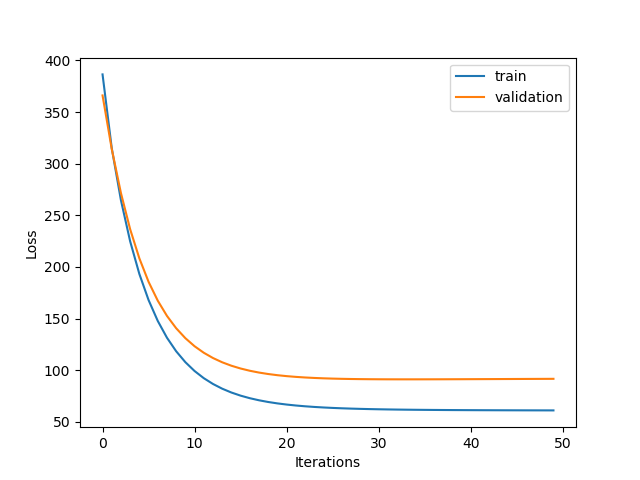
\includegraphics[scale = 0.5]{"../output/linear_classifier.png"}

    The val loss was $71.8$ and the train loss was $68.7$. I did not use this baseline on the test data as I am holding that out till I have a more refined model.

    The code for my work so far is available at https://github.com/seanroelofs/covid-by-county


\section{Next Steps}

    Since the validation loss and train loss were so close on my linear regressor, I predict that my current model is underfiting the data. I have good hope that a more sophisticated neural network model will be able to perform better on this task.

    For my next steps, I plan to implement a NN model in PyTorch. I will tune the structure and hyperparameters of the network using ideas from this class.

    I will also plan to find a better metric in which to define the rate of infection instead of the $5$ to $50$ day metric currently in use. I think this metric may be noisy and does not use the full representative power of the NYT dataset. Perhaps the growth rate on an exponentially fitted curve of cases for each county would be a better label.

\section{Sources}

1. Coronavirus Disease 2019. Centers for Disease Control and Prevention. cdc.gov/coronavirus/2019-ncov/cases-updates/cases-in-us

2. US Census Demographic Data. US Census Bureau. kaggle.com/muonneutrino/us-census-demographic-data

3. Coronavirus (Covid-19) Data in the United States. The New York Times. github.com/nytimes/covid-19-data

\end{document}
